% !TeX root = ../Book2.tex
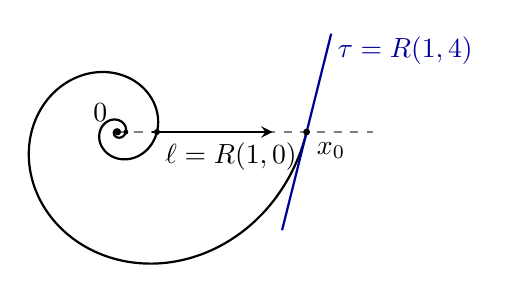
\begin{tikzpicture}[scale=2.4,>=stealth,line width=.8pt]
	\draw[smooth,samples=500,domain=-1440:0,variable=\a] plot ({exp(\a*pi/720)*cos(\a)},{exp(\a*pi/720)*sin(\a)});
	\draw[dashed,gray] (0,0)--(1.35,0);
	\draw[->,thick] (.18,0)--(.82,0);
	\draw[blue!60!black] (.87,-.52)--(1.13,.52);
	\fill (0,0) circle (.018) node[above left] {\(0\)};
	\fill (1,0) circle (.018) node[below right] {\(x_0\)};
	\fill ({exp(-pi/2)},0) circle (.016);
	\fill ({exp(-pi)},0) circle (.013);
	\node[below] at (.60,0) {\(\ell=\mathbb R(1,0)\)};
	\node[right,blue!60!black] at (1.11,.43) {\(\tau=\mathbb R(1,4)\)};
\end{tikzpicture}
